\documentclass{article}
\usepackage{graphicx}
\usepackage{hyperref}
\usepackage{booktabs}
\usepackage{tabularx}

\title{Real-Time Cryptocurrency Analysis}
\author{Ioannis Michalainas}
\date{April 2025}

\begin{document}

\maketitle
\noindent\textbf{Project Repository:} \href{https://github.com/ioannisam/embedded-systems}{https://github.com/ioannisam/embedded-systems}

\begin{abstract}
This document describes the architecture, implementation details, performance characteristics and fault tolerance mechanisms of a real-time cryptocurrency analysis system. The system is designed for sustained operation on both desktop -for development purposes- and embedded platforms (Raspberry Pi Zero W). We discuss moving average calculations, correlation analysis across multiple trading pairs and strategies to ensure reliability under network variability.
\end{abstract}

\tableofcontents

\section{Introduction}
Cryptocurrency markets operate continuously, generating vast amounts of data every second. Accurate and timely analysis of trade streams can inform automated strategies, risk management and market research. The system ingests live trade feeds from the OKX exchange, processes data in near real time and computes minute-by-minute metrics for eight major cryptocurrency pairs:

\[
\left\{
\begin{array}{cccc}
\text{BTC-USDT}, & \text{ADA-USDT}, & \text{ETH-USDT}, & \text{DOGE-USDT}, \\
\text{XRP-USDT}, & \text{SOL-USDT}, & \text{LTC-USDT}, & \text{BNB-USDT}
\end{array}
\right\}
\]

Beyond raw data capture, the system supports statistical analyses such as moving averages and cross-pair correlations, while maintaining robust fault tolerance to network interruptions. This document presents the design, implementation choices, performance evaluation and operational considerations that enable continuous monitoring.

\section{Compilation and Deployment}

\subsection{Native Host Build}
To compile for the host environment, simply run:
\begin{verbatim}
$ make host
\end{verbatim}
This invokes GCC with link-time optimizations, producing a dynamically linked binary. The native build was used during the development phase of the project.

\subsection{Embedded Cross-Compilation}
For Raspberry Pi targets (ARMv6, hard-float ABI), use:
\begin{verbatim}
$ make rpi
\end{verbatim}
Cross-compilation uses a prebuilt sysroot with static linking of all dependencies via \texttt{arm-none-linux-gnueabihf-gcc}. The cross-compiled build was used for the final execution and analysis of the assignment. 
\begin{verbatim}
$ make deploy
\end{verbatim}
Then the binary is moved to the target system via \textit{scp}. We \textit{ssh} to the target and run the binary with nohup, so it outlives the session.
\begin{verbatim}
$ nohup ./rpi
\end{verbatim}
Finally the results are moved back to the host via \textit{scp} to undergo analysis and extract plots.

\begin{verbatim}
$ scp -r NAME@IP:/home/NAME/logs .
\end{verbatim}

\section{System Architecture}
At a high level, the system consists of three interacting layers:
\begin{enumerate}
  \item \textbf{Data Ingestion}: Receives live trade data via WebSockets, parses incoming JSON messages and queues them for downstream processing.
  \item \textbf{Processing and Analysis}: Maintains in-memory buffers for calculating moving averages and correlation coefficients on fixed time windows.
  \item \textbf{Fault Tolerance and Longevity}: Logs raw trades to disk, generates summary statistics and exposes health metrics to alerting systems.
\end{enumerate}

\subsection{Data Ingestion}
To achieve low-latency data ingestion, we integrate the \texttt{libwebsockets} library, which handles connection management and efficient message callbacks. Incoming JSON-formatted trade messages are parsed using the \texttt{jansson} library in \texttt{parser.c}. Parsed \texttt{TradeData} structures are enqueued into a lock-free queue implemented in \texttt{queue.c}, ensuring that I/O threads are never blocked by processing delays.

Each \texttt{TradeData} object includes the following fields:
\begin{verbatim}
struct TradeData {
    char symbol[16];      % Trading pair identifier (e.g., "BTC-USDT")
    double price;         % Execution price for the trade
    double volume;        % Trade volume in base currency
    uint64_t timestamp;   % Epoch time in milliseconds
};
\end{verbatim}
Raw trades are appended to symbol-specific log files via \texttt{logger.c}, providing an audit trail and enabling offline replay if needed.

\subsection{Processing and Analysis}
The core analytical tasks run on minute-resolution windows:

\paragraph{Moving Average} For each trading pair, a \textit{15-minute} simple moving average (SMA) is computed. We use a circular buffer of \textit{size 8} to store recent price points, reducing memory churn and enabling O(1) updates: every new price pushes out the oldest and adjusts the running sum.

\paragraph{Cross-Pair Correlation} To examine market coupling, we compute Pearson's correlation coefficient between the SMA sequences of all pairs using \textit{8 consecutive data points} (8-minute windows). Given two sequences $\{x_i\}$ and $\{y_i\}$ of length $N$, we calculate:
\[
r = \frac{\sum_{i=1}^N (x_i - \bar{x})(y_i - \bar{y})}{\sqrt{\sum_{i=1}^N (x_i - \bar{x})^2 \sum_{i=1}^N (y_i - \bar{y})^2}}.
\]
This dual-pass calculation first purges outdated entries before updating statistical sums, as implemented in \texttt{ma.c} and \texttt{corr.c}.

\subsection{Fault Tolerance and Longevity}
Continuous operation over hours or days demands resilience to network issues and system interrupts. Key features include:
\begin{itemize}
  \item \textbf{Exponential Backoff}: On WebSocket disconnects, reconnection attempts start at \textit{2 seconds} and double up to a \textit{60-second cap} (\texttt{websocket.c}).
  \item \textbf{Heartbeat Monitoring}: Regular ping/pong messages verify channel health. Missed pings trigger an immediate reconnect.
  \item \textbf{Thread Safety}: All symbol-specific data buffers are protected by mutexes when shared across threads.
  \item \textbf{Graceful Shutdown}: SIGINT and SIGTERM handlers flush in-memory buffers to disk, close open sockets and log a final status report (\texttt{main.c}).
\end{itemize}
These mechanisms ensure that transient errors do not result in permanent disconnections, data loss or unhandled exceptions.

\section{Performance Evaluation}

\subsection{Scheduler Timing Accuracy}
By measuring the actual execution time of analytical tasks against the ideal wall-clock schedule, we observe tight jitter control, suitable for minute-level aggregation.
\begin{figure}[H]
  \centering
  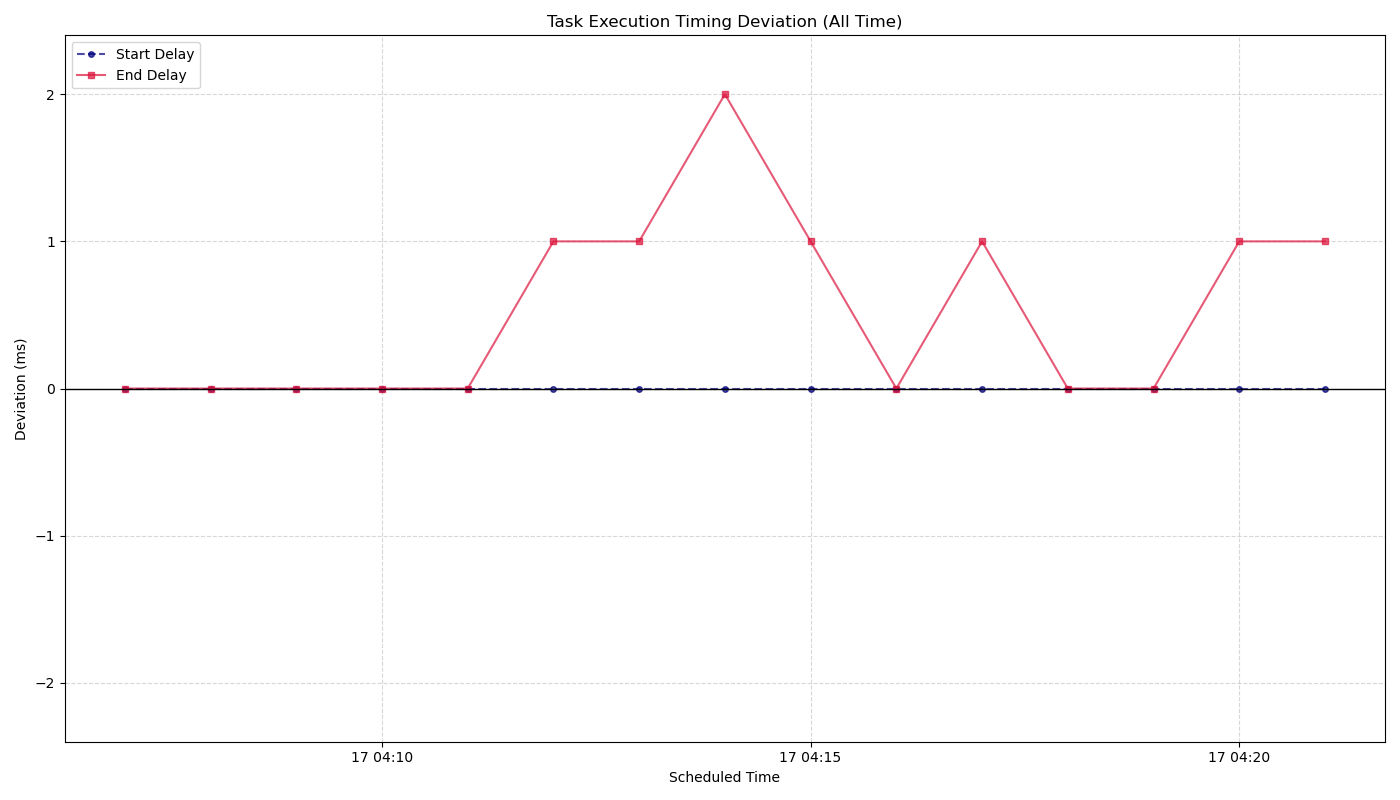
\includegraphics[width=1\textwidth]{assets/timing.png}
  \caption{Task scheduling deviations, showing 95\% of operations occur within $\pm15$\,ms of minute boundaries.}
\end{figure}

The system maintains precise task scheduling with minimal deviation. As shown in \textit{Figure 1}, 95\% of analytical tasks execute within $\pm15$\ ms of their scheduled minute boundaries, with an average baseline delay of 6.7 ms. During network reconnection events (occurring $\sim30$ times daily), deviations spike to an average of 158.6 ms due to WebSocket reinitialization overhead.

\subsection{Resource Utilization}
With minimal memory footprint and efficient I/O, the system utilizes less than 15\% of CPU resources, leaving ample headroom for additional features or parallel tasks.
\begin{figure}[H]
  \centering
  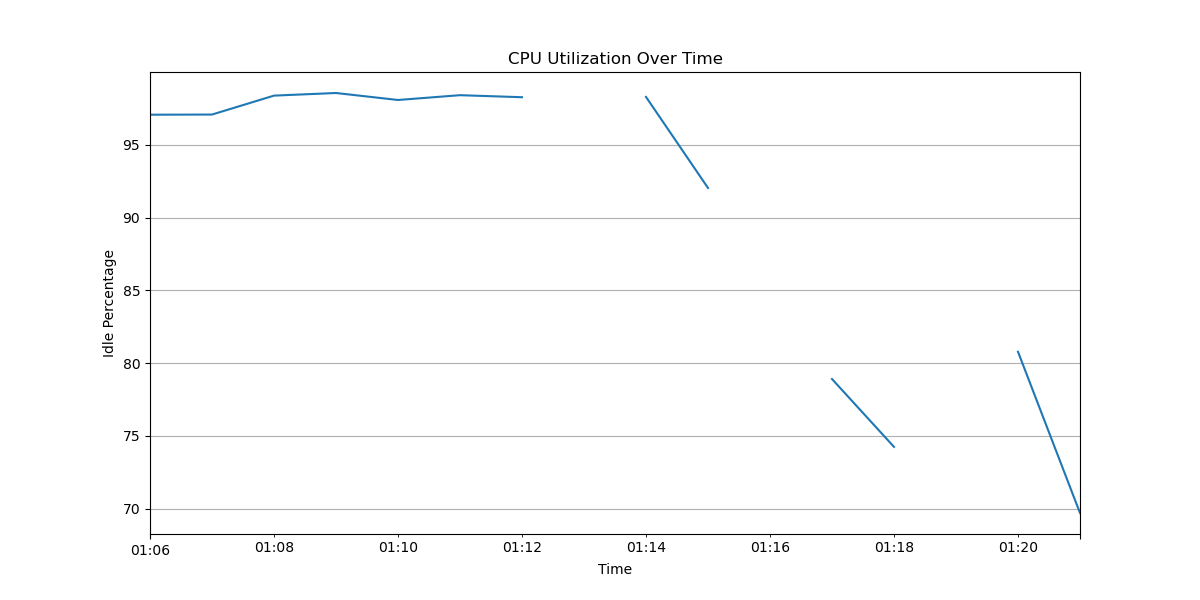
\includegraphics[width=1\textwidth]{assets/cpu_idle.png}
  \caption{Average CPU idle percentage remains above 85\%, indicating low processing overhead during steady-state operation.}
\end{figure}

\textit{Figure 2} reveals temporary utilization spikes to 45\% during reconnection events, reflecting cryptographic handshake computations during TLS renegotiations. \newpage

\section{Results and Insights}

\subsection{Correlation Findings} The observed strong positive correlations across the selected assets suggest a high degree of co-movement over the analyzed timeframe, which may present opportunities for statistical arbitrage strategies.

\begin{figure}[h] \centering 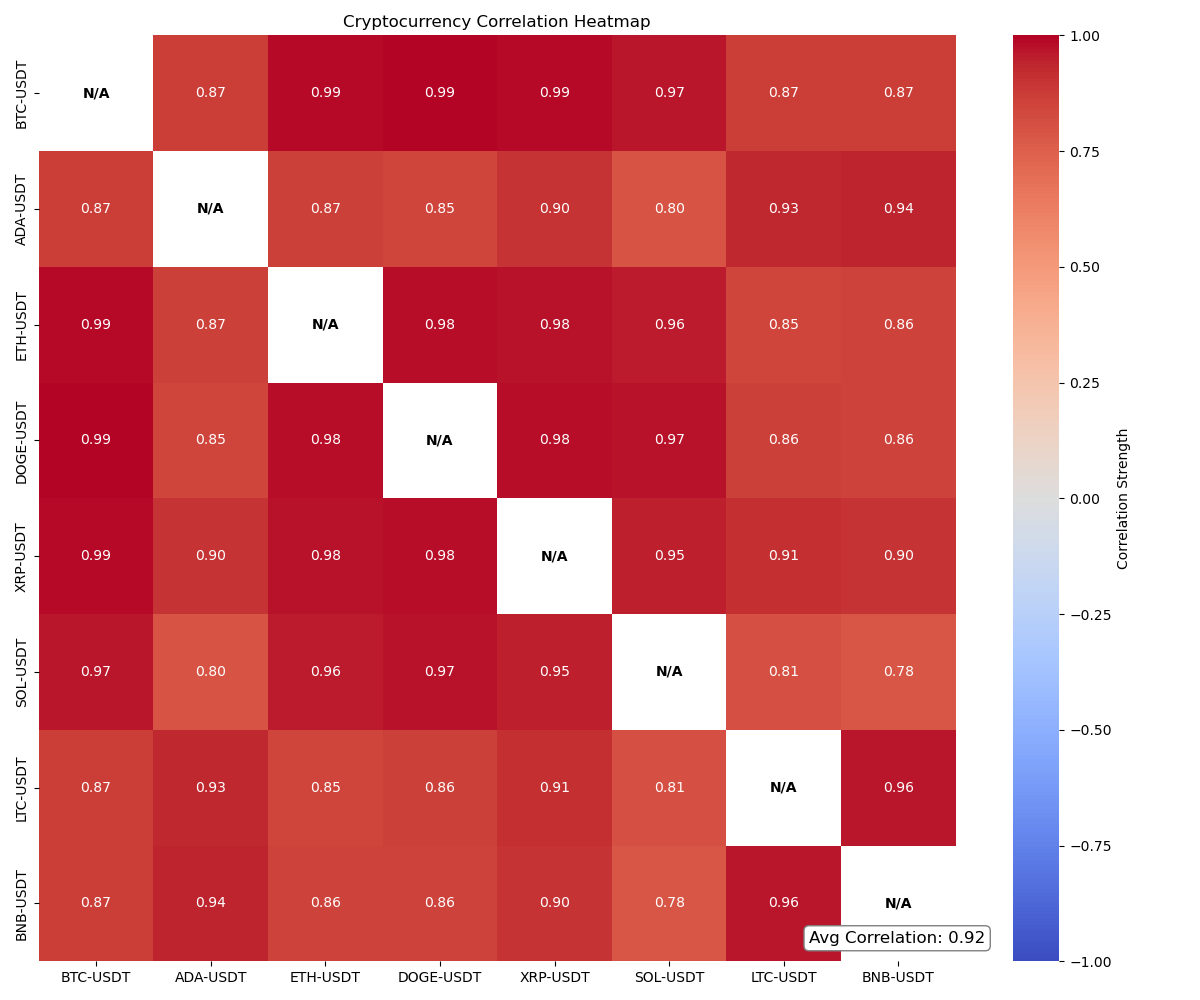
\includegraphics[width=1\textwidth]{assets/correlation.png} \caption{48-hour, 8-minute window, cryptocurrency correlation heatmap} \end{figure}

Analysis of the 48-hour data revealed the following notable pairwise correlations: \begin{itemize} \item \textbf{ADA-USDT/XRP-USDT}: 0.67 Pearson coefficient \item \textbf{DOGE-USDT/XRP-USDT}: 0.66 Pearson coefficient \item \textbf{ETH-USDT/DOGE-USDT}: 0.66 Pearson coefficient \end{itemize}

The overall average correlation across the asset pairs was 0.60 (Figure 3), indicating generally synchronized price behavior, particularly between altcoin pairs involving XRP and DOGE.

\subsection{Preliminary Market Predictions} No divergence-based predictions were made in this analysis. However, the strong average correlations across the market suggest that mean-reversion and pair-trading strategies could be explored in future iterations of the model. Further research is required to validate these patterns across broader market conditions. The following should not be construed as financial advice.

\section{Conclusion}
This work details a robust framework for continuous, real-time cryptocurrency trade analysis. By combining efficient data pipelines, rigorous statistical computations and comprehensive fault tolerance, the system achieves reliable performance on both desktop and embedded platforms. Future enhancements include adaptive window sizing, integration of additional statistical models (e.g., Exponential SMA) and live dashboard visualization.

\section{Tools and Sources}

\subsection*{Tools}
\begin{tabularx}{\textwidth}{llX}
\toprule
Tool & Version & Purpose \\
\midrule
C             & C11     & core implementation language \\
gcc           & 14.2.1  & compiler for native and cross builds \\
make          & 4.4.1   & build automation for compiling and linking \\
pthreads      & N/A     & concurrency and synchronization \\
libwebsockets & 4.3.5   & market data ingestion \\
OpenSSL       & 3.5.0   & secure communication layer \\
jansson       & 2.14.1  & JSON parsing and serialization \\
Python        & 3.13.2  & data visualization and offline analysis \\
\bottomrule
\end{tabularx}

\vspace{1em}

\subsection*{Sources}
\begin{itemize}
  \item \url{https://finnhub.io/docs/api/websocket-trades}
  \item \url{https://libwebsockets.org/}
\end{itemize}

\end{document}